%\documentclass[times, 11pt, onecolumn]{article} 
%\documentclass[times, 10pt]{article} 
%\documentclass{article} 

\documentclass[conference,final]{IEEEtran}

\usepackage{latex8}
\usepackage{times}

\usepackage[utf8]{inputenc}
\usepackage{graphicx}
\usepackage{url}
\usepackage{float}
\usepackage{times}    
\usepackage{multirow}    
\usepackage{listings}   
\usepackage{times}     
\usepackage{paralist}    
\usepackage{wrapfig}    
\usepackage[small,it]{caption}
\usepackage{multirow}
\usepackage{ifpdf}
\usepackage{subfigure}

\usepackage{listings}
\usepackage{keyval}  
\usepackage{color}
\definecolor{listinggray}{gray}{0.95}
\definecolor{darkgray}{gray}{0.7}
\definecolor{commentgreen}{rgb}{0, 0.4, 0}
\definecolor{darkblue}{rgb}{0, 0, 0.4}
\definecolor{middleblue}{rgb}{0, 0, 0.7}
\definecolor{darkred}{rgb}{0.4, 0, 0}
\definecolor{brown}{rgb}{0.5, 0.5, 0}

\lstdefinestyle{myListing}{
  frame=single,   
  backgroundcolor=\color{listinggray},  
  %float=t,
  language=C,       
  basicstyle=\ttfamily \footnotesize,
  breakautoindent=true,
  breaklines=true
  tabsize=2,
  captionpos=b,  
  aboveskip=0em,
  belowskip=-2em,
  %numbers=left, 
  %numberstyle=\tiny
}      

\lstdefinestyle{myPythonListing}{
  frame=single,   
  backgroundcolor=\color{listinggray},  
  %float=t,
  language=Python,       
  basicstyle=\ttfamily \footnotesize,
  breakautoindent=true,
  breaklines=true
  tabsize=2,
  captionpos=b,  
  %numbers=left, 
  %numberstyle=\tiny
}

\newcommand{\up}{\vspace*{-1em}}
\newcommand{\upp}{\vspace*{-0.5em}}


\title{
  ~\\[-3em]
  Developing Applications With Loosely-Coupled Sub-Tasks Using a
  Standard Programmatic Interface}

  \author{
    ~\\[-2em]
    % Unsure of Author List$^{1}$ \\
    Shantenu Jha$^{1,2,3}$, Yaakoub El-Khamra$^{1}$, Joohyun Kim$^{1}$,
    Andre Luckow$^{4}$, \\
    \small{\emph{$^{1}$Center for Computation \& Technology, Louisiana State University, USA}}\\
    \small{\emph{$^{2}$Department of Computer Science, Louisiana State
        University, USA}}\\
    \small{\emph{$^{3}$e-Science Institute, Edinburgh, UK}}\\
    \small{\emph{$^{4}$Institute of Computer Science, Potsdam University, Germany}}\\
  }
%\date{}

\def\acknowledgementname{Acknowledgements}

\newenvironment{acknowledgement}%

{\section*{\acknowledgementname}%
\parindent=0pt%
}

\newif\ifdraft
\drafttrue
\ifdraft
\newcommand{\kimnote}[1]{ {\textcolor{green} { ***JK: #1 }}}
\newcommand{\alnote}[1]{ {\textcolor{blue} { ***AL: #1 }}}
\newcommand{\amnote}[1]{ {\textcolor{magenta} { ***AM: #1 }}}
\newcommand{\jhanote}[1]{ {\textcolor{red} { ***SJ: #1 }}}
\else
\newcommand{\kimnote}[1]{}
\newcommand{\alnote}[1]{}
\newcommand{\amnote}[1]{}
\newcommand{\jhanote}[1]{}
\fi

\begin{document} 


\maketitle    

\begin{abstract}
  The Simple API for Grid Applications (SAGA) can be used to
  programmatically develop a very wide-range of distributed
  applications.  In this paper we describe how SAGA has been used to
  develop two different applications from the following classes of
  distributed applications (i) applications based upon the loose
  coupling of homogenous sub-tasks and, (ii) applications based upon
  loose coupling of simulations of heterogenous sub-tasks.  The nature
  of the coupling also varies significantly for these applications,
  and plays an important role in the development and deployment
  options available.  The specific applications developed are
  Replica-Exchange simulations using Molecular Dynamics and
  Kalman-Filter based application for reservoir simulation.  We
  briefly discuss the specific applications developed and the typical
  science problems tackled using these applications.  We will describe
  the application characteristics of the two case-studies, with a
  focus on the distributed logic of these simulations, and not the
  core simulation logic of the applications.  The paper analyses and
  contrasts the application characteristics of the examples, and shows
  how they are supported using SAGA, often in conjunction with other
  programming frameworks such as Cactus. Along with the development of
  multi-task applications, it is also important to focus on the
  deployment challenges, especially if, as we will argue that the
  dynamic applications (which form an important class of applications
  with multi-tasks) in addition to requiring programming models tht
  support explicit distributed, must also have an agile execution
  model.  The primary aim of this paper is to demonstrate how SAGA can
  be an effective tool for programmatically representing and
  implementing the logic of coordination and orchestrating multiple,
  distributed tasks, while remaining agnostic to the actual mechanism,
  ie. details of the distributed environment. We will highlight the
  importance of programming abstractions and how frameworks that
  provide common programming patterns can be used to simplify the
  construction of distributed applications.
\end{abstract}

The story is as follows. 

We have two distinct applications -- REMD and a Kalman-Filter based
applications.

These applications are prototypes of two important applications
classes -- loosely coupled multiple identical sub-tasks (ie replicas)
and multiple, loosely-coupled but heterogenous sub-tasks.  (In the
latter case, they are not only heterogenous they are also highly
irregular).  We have demonstrated that these applications work
perfectly well in distributed environments.

The aim of this paper is to demonstrate that these applications can be
deployed and executed on high-end machines, using exactly the same
framework, ie, there exists a standard, programmatic approach to
codify these applications such that they can be seamlessly run on any
underlying infrastructure. Critically this implies that the the
application developer focusses on supporting the application
characteristics and not worrying about the details of the underlying
infrastructure.

Although both are classified as loosely-coupled, the nature of the
coupling between the sub-tasks varies. We posit that along with the
size and number of sub-tasks, the coupling between the sub-tasks is an
important determinant of the development and deployment mechanism.

In the former, the sub-tasks
progress independent of other sub-tasks with the exception of one
(referred to as the paired replica). There is a pair-wise exchange of
some parameters after a certain time-period (maybe fixed or not), and
it is possible that the paired-replicas differ, i.e., a replica is
paired with a different replica as time progresses. If the sub-task
that a replica is paired with is not is not ready for exchange, the
sub-tasks goes into a wait state, i.e., the consequence of
load-balancing is typically localized to the paired replica. If there
are multiple replicas in a wait state, sophisticated scheduling can be
invoked to progress waiting tasks. \jhanote{elaborate a bit}

It is important to contrast this ``coupling'' with the coupling in the
latter application's (Kalman Filter) case. For the Kalman-Filter
application, the multiple sub-tasks need to {\it all} complete
as there is a global synchronization point, and the output
of all sub-tasks are required to generate the input for the next
stage.

It is important to appreciate the nature of the coupling of the
sub-tasks, as it imposes constraints on the (i) scheduling strategies,
(ii) speculative computing (iii) resource mapping strategies, and thus
the deployment strategy.

As we will go onto discuss, it is often the problems associated with
deployment on production general-purpose Grids (ie brod-Grids) using
general purpose grid infrastructure that makes the uptake of grids
challenging and often unattractive to the end-scientists. In a
nutshell, deployment is more difficult as Grids systems are comprised
of many ``isolated'' components and we believe that this contributes
to currently unmanagable number degrees-of-freedom and failure modes.
Thus, although programming models and conceptual frameworks exists to
unify the uptake of ``grids or supercomputers'' as required, practical
considerations make this currently unrealistic and motivate the
end-scientist to settle for the the solution that is often simpler to
deploy. 

\jhanote{The bulk of the next three sections should be pretty much a
  cut and paste job. What is really required is i. run the multi-tasks
  of the kalman filter application entirely on Abe ii. run the
  multi-tasks of the replica exchange entirely on Abe}

\jhanote{Although they belong to different classes, we show here that
  they can be deployed effectively on i) Range of systems and scales,
  a smaller but many distributed systems as well as a single, but much
  larger top-end system. ii) Explicitly versus Implicitly: dynamic
  applications profit from being able to have.....}

\jhanote{Need to talk about algorithms that can be decomposed
  spatially, but retain a level of synchronisation, between stages,
  There is a challenge in the scheduling of the sub-tasks.  This is
  probably a general challenge/problem of ``many tasks'' computing;
  there isn't always a need for tight co-scheduling, but a need for
  some level of loose coupled scheduling.  Some level of best effort
  resource allocation is acceptable.}

\section{SAGA: A Standard Programming Interface}


\begin{figure}[!h]
  \begin{center}
    \subfigure{\label{sagalayer1}
      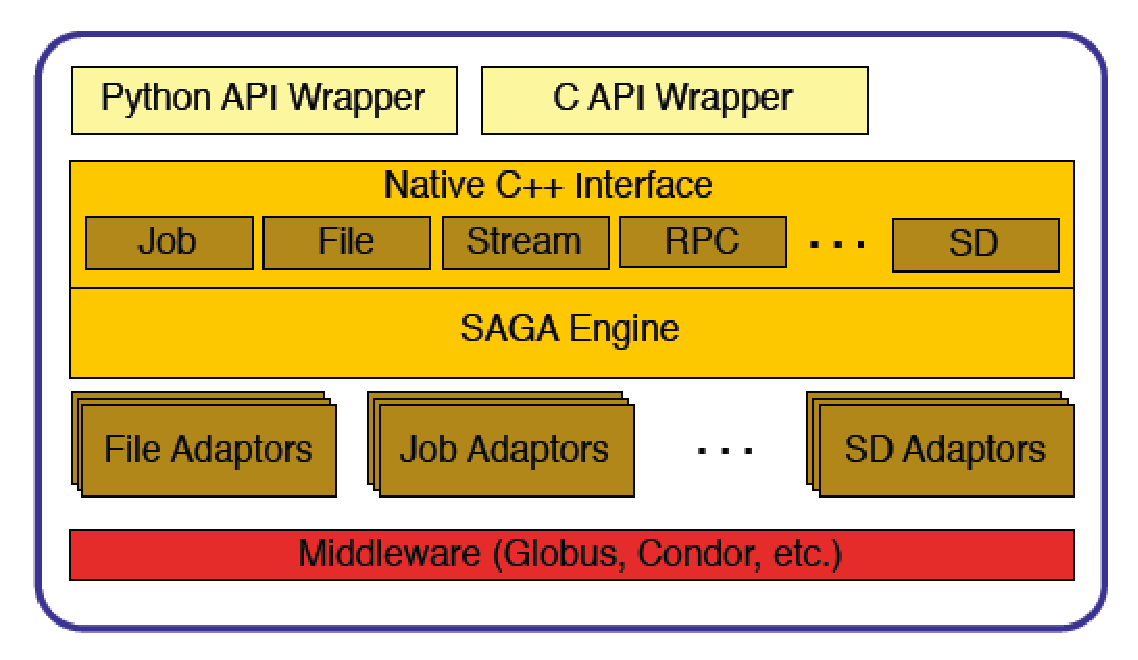
\includegraphics[width=3.55in]{saga_layered_landscape}}     
%     \subfigure{\label{sagalayer2}
%       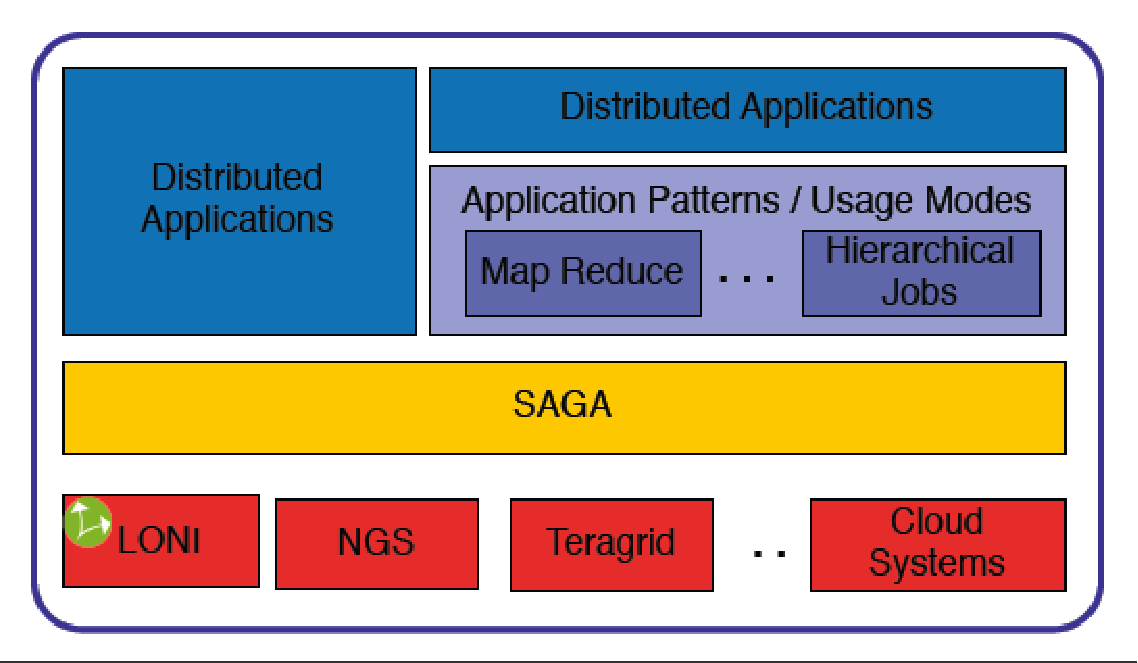
\includegraphics[width=3.55in]{saga_layered_application}}
  \end{center}
  \caption{Layered schematic of the different components of the SAGA
    landscape.  Middleware specific adaptors applications developed
    using SAGA make applications developed using SAGA grid
    portable. Schematic showing the different ways in which SAGA can
    be used to develop distributed applications}
 \label{sagalayer}
\end{figure}

The Simple API for Grid Applications (SAGA) is an API standardization
effort within the Open Grid Forum (OGF)~\cite{ogf_web} an
international standards development body concerned primarily with
standards for distributed computing.  SAGA provides a simple,
POSIX-style API to the most common Grid functions at a sufficiently
high-level of abstraction so as to be able to be independent of the
diverse and dynamic Grid environments.  The SAGA specification defines
interfaces for the most common Grid-programming functions grouped as a
set of functional packages.  Version 1.0~\cite{saga-core} of the
specification has been submitted to the OGF editorial pipeline.  It
defines the following packages:

\begin{itemize}
\item File package - provides methods for accessing local and remote
  filesystems, browsing directories, moving, copying, and deleting
  files, setting access permissions, as well as zero-copy reading and
  writing
\item Replica package - provides methods for replica management such
  as browsing logical filesystems, moving, copying, deleting logical
  entries, adding and removing physical files from a logical file
  entry, and search logical files based on attribute sets.
\item Job package - provides methods for describing, submitting,
  monitoring, and controlling local and remote jobs. Many parts of
  this package were derived from the largely adopted
  DRMAA~\cite{drmaa_url} specification.
\item Stream package - provides methods for authenticated local and
  remote socket connections with hooks to support authorization and
  encryption schemes.
\item RPC package - is an implementation of the GGF GridRPC
  API~\cite{gridrpc_url} definition and provides methods for unified
  remote procedure calls.
\end{itemize}

The two critical aspects of SAGA are its {\it simplicity} of use and
the fact that it is well on the road to becoming a community {\it
  standard}.  It is important to note, that these two properties
provide the added value of using SAGA for Grid application
development.  Simplicity arises from being able to limit the scope to
only the most common and important grid-functionality required by
applications.  Standardization represents the fact that the interface
is derived from a wide-range of applications using a collaborative
approach and the output of which is endorsed by the broader community.


\begin{figure}[!h]
  \begin{center}
%     \subfigure{\label{sagalayer1}
%       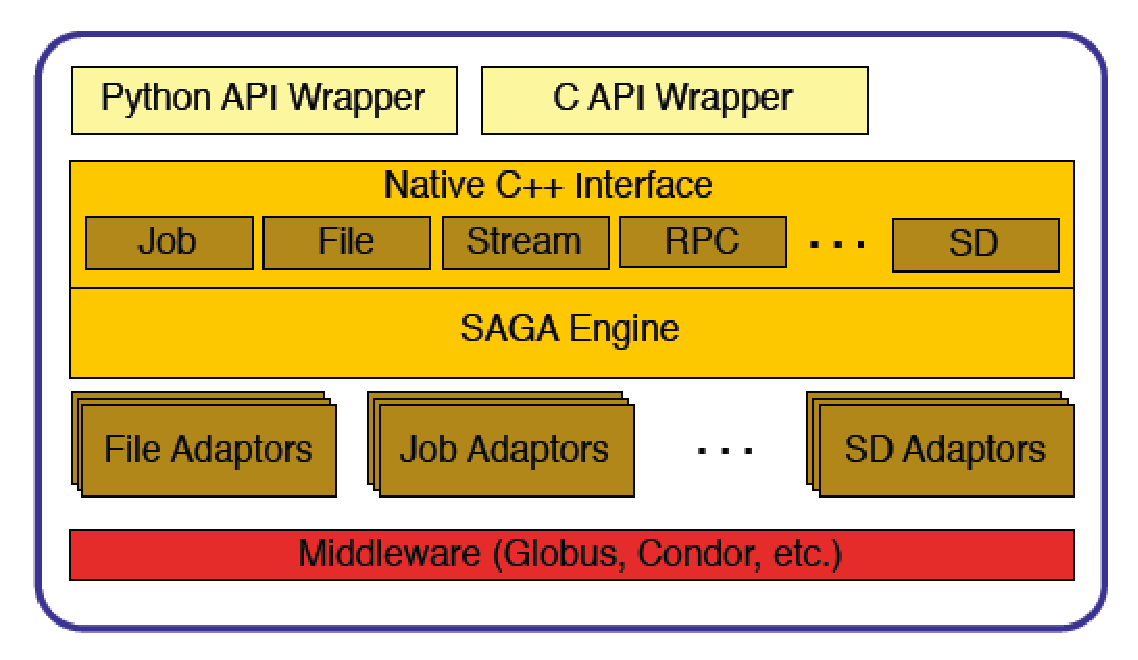
\includegraphics[width=3.55in]{saga_layered_landscape}}     
    \subfigure{\label{sagalayer2}
      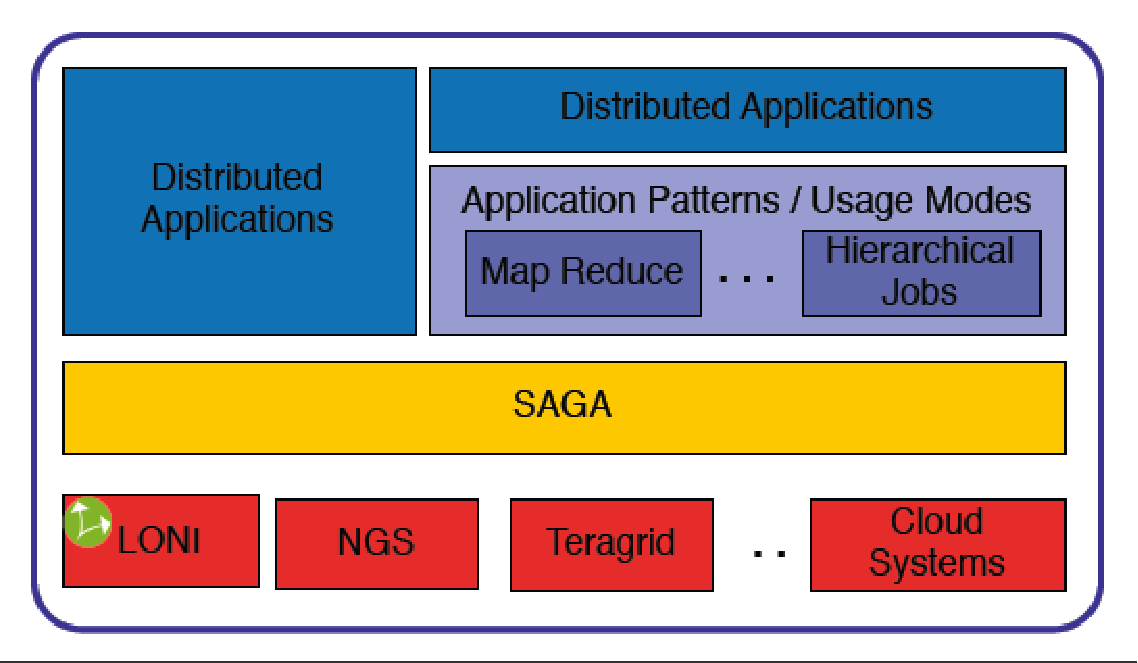
\includegraphics[width=3.55in]{saga_layered_application}}
  \end{center}
  \caption{Layered schematic of the different components of the SAGA
    landscape.  Middleware specific adaptors applications developed
    using SAGA make applications developed using SAGA grid
    portable. Schematic showing the different ways in which SAGA can
    be used to develop distributed applications}
 \label{sagalayer}
\end{figure}


\section{Applications With Loosely-Coupled Homogeneous
  Sub-Tasks: Replica-Exchange Simulations}  

\alnote{Are we referring to sub-jobs as sub-tasks or sub-job? Just to
  keep this consistent with the other paper. We previously discussed
  that task has another meaning within SAGA, which could potentially
  lead to confusion.}
  
\jhanote{Andre, the word to avoid is ``tasks'', which is the term that
  has a SAGA specific context. I think we can safely use sub-tasks for
  sub-jobs if we like to. Especially given that the workshop is using
  a generic term -- ``multi-tasks''.}

An example for a distributed application consisting of homogeneous
sub-tasks are Replica-Exchange (RE) simulations~\cite{Sugita:1999rm},
\cite{hansmann}. Such applications can be used to understand important
physical phenomena -- ranging from protein folding dynamics to binding
affinity calculations required for computational drug discovery.  For
Replica-Exchange simulations utilizing as many distributed resources
as possible, is critical for the effective solution of the scientific
problem~\cite{repex_ptrsa}.

Distributed RE simulations must be able to orchestrate different
resources in a complex and dynamic environment.  Writing such an
applications is a complex task for a myriad number of reasons, not
least of which is that distributed computing environments are
inherently prone to failures. In the following the SAGA-based RE
framework developed for molecular dynamics simulations is described.

\subsection{Application Description}

Replica-exchange simulations are also used to allow a sufficient
sampling of configurations. This is an important requirement for
connecting atomistic results to macroscopic or thermodynamic
quantities available from experiments.  However, even with the most
powerful computing resources at the moment, straight-forward MD
simulations are unable to reach the relevant time-scales required to
study conformational changes and searches. This is partly due to the
inherent limitations in the MD algorithm -- a global synchronization
is required at the end of each time step.  This provides an important
motivation for research into finding ways to accelerate sampling and
enhance ``effective'' time-scales studied. Generalized ensemble
approaches -- of which Replica-Exchange Molecular Dynamics
(REMD)~\cite{Sugita:1999rm} are a prominent example -- represent an
important and promising attempt to overcome the general limitations of
insufficient time-scales, as well as specific limitations of
inadequate conformational sampling arising from kinetic trappings.  In
the simplest formulation, Replica-exchange is an algoirthm whereby one
single long-running simulation is be substituted for an ensemble of
shorter-running similar simulations, but which are very
loosely-coupled, ie, the interval between exchange attempts is much
larger than the interval over which the simulations run; this also
make the replica-exchange formulation of physical problems excellent
candidates for distributed environments.

%\section{Replica Exchange Simulations}
% Replica Exchange simulations used within Molecular Dynamics (MD)
% approaches,

\subsection{Application Architecture}

\alnote{Should I mention CPR/Migol or should I rather keep it on the
  ``abstractions'' level?}  Replica-Exchange (RE) simulations can be
thought of as consisting of two distinct components: the simulation
engine/mechanism used for each replica process, and the
coupling-mechanism between the individual replicas. The RE framework
relies NAMD as MD code for carrying out the simulation and a
SAGA-based framework for orchestration of the replica sub-tasks.

The developed RE framework~\cite{Luckow:2008la} comprises of the
\emph{RE-Manager}, the central master deployed on the user's desktop,
and the \textit{Replica-Agents}, that reside on the High Performance
machines where RE simulations are carried out. The RE-Manager
orchestrates all replicas, i.\,e.\ it is responsible for the
parameterization of replica tasks, file staging, job spawning and the
conduction of the replica-exchange itself.  The Replica-Agent is
launched by a Grid job and is responsible for spawning and monitoring
the replica processes.

Figure~\ref{fig:remdmanager_v11} summarizes the abstractions used
within the RE framework.  For file management the RE-Manager utilizes
the SAGA File API. More complex, is the management of replica
sub-jobs. To achieve an optimal time to solution an efficient
dispatching of the RE sub-jobs is required.

\begin{figure}[htbp]
    \centering
        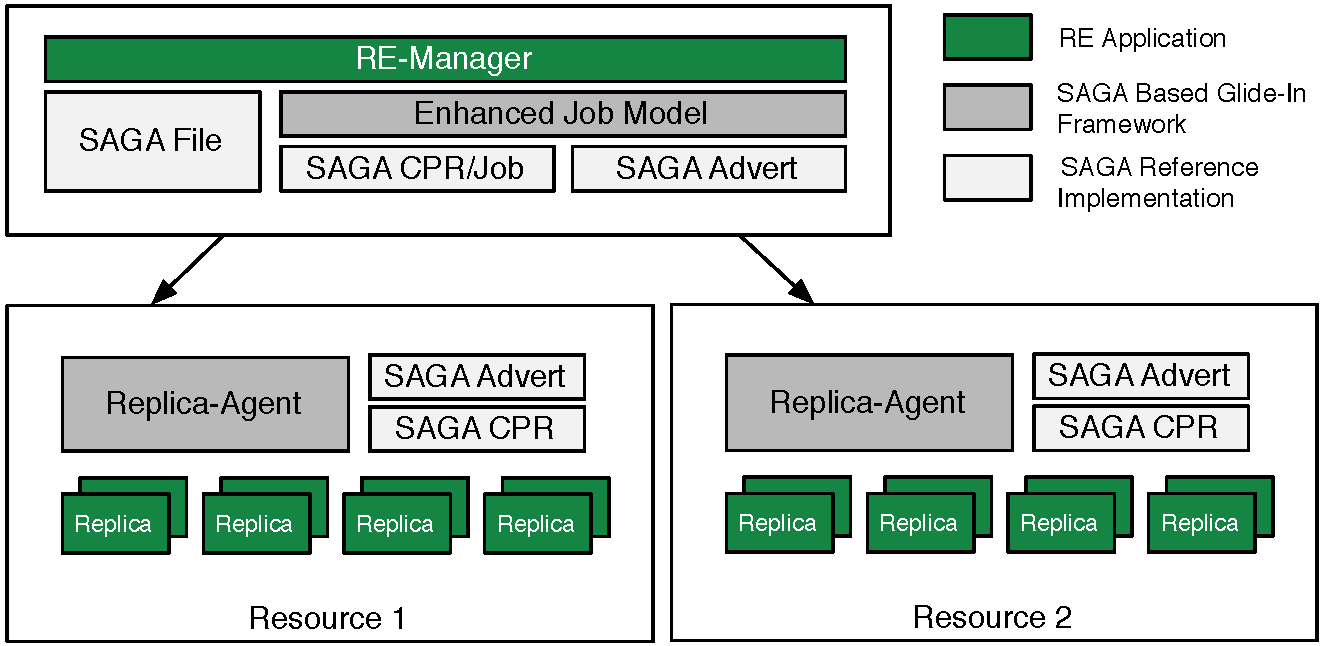
\includegraphics[width=0.45\textwidth]{remdmanager_v11.pdf}
    \caption{Replica Exchange Framework Abstractions:      
          The Replica-Agent is used as placeholder job for
          all replica sub-jobs running on a single cluster. The
          RE-Manager can control both the Replica-Agents and the replica
          jobs using a SAGA-based user-level job API. By using this
          efficient way to allocate resources, queuing times are minimized
          and the time to completion can be dramatically reduced.}
    \label{fig:remdmanager_v11}
\end{figure}  

In particular, queueing delays can represent a major bottleneck: a
single crowded resource can slowdown the simulation arbitrary. A
common principle to prevent this is the usage of Glide-In jobs, which
represent a placeholder for a set of sub-jobs (see Frey
et.\,al.~\cite{citeulike:291860}).  For this Glide-In job a
sufficiently large chunk of resources is requested. Smaller sub-jobs
can then rapidly be executed through the Glide-In job.

The SAGA Glide-In framework comprises of two components: 1) The
Glide-In manager provides the enhance job model API and allows the
management of both Glide-In jobs and sub-jobs.  2) The Replica-Agents
represent the Glide-In jobs. The agents manage their allocated
resources and dispatch sub-jobs on request. In this sense the
Replica-Agents implement the functionality of an application-level
scheduler. Communication between the Replica-Agent and Glide-In
manager is carried out using the SAGA advert service, a central
key/value store.

With this capability the SAGA Glide-In framework provides a novel
system-level abstraction for allocating larger chunks of resources and
for mapping these resources to a set of sub-jobs. The enhanced job
model can be used as drop-in replacement for a SAGA job objects. No
code modification is required -- the application must solely map the
sub-jobs to a suitable Glide-In job.  The RE-Manager relies on the
SAGA Glide-In framework to reserve resources on a cluster and to
efficiently dispatch RE processes to these nodes.

While the implementation of the enhanced job model is entirely based
on SAGA and in particular the SAGA Advert Service, a central key/value
store, a utilization of other frameworks, such as the orignal Condor
Glide-In~\cite{citeulike:291860} or Falcon~\cite{1362680}, is
possible. Currently, we are actively working on a Condor adaptor for
SAGA, which will also support native Glide-In functionality for Condor
Jobs; our enhanced job model will then serve as abstraction, while the
Condor level Glide-In is used as implementation where appropriate.

\section{Applications With Loosely-Coupled Heterogenous
Sub-Tasks: Kalman-Filter Based Simulations}

\subsection{Application Description}

% \subsection{SAGA and Cactus: A Powerful Application Development
%   Framework}

% \subsection{Deploying on Distributed Resources}

% \subsection{Deploying on Abe}

% BQP used for the first time to dynamically determine queue and model
% size within a given system to submit sub-task to...
%\section{}

\begin{figure}[htbp]
    \centering
    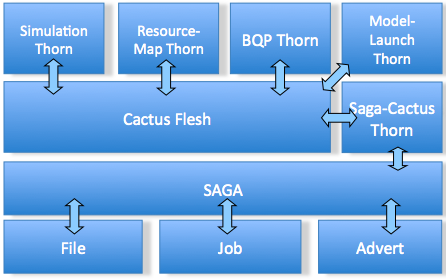
\includegraphics[width=0.45\textwidth]{kalmanfilterlayer.pdf}
    \caption{}
    \label{fig:remdmanager_v11}
\end{figure}  

Ensemble Kalman filters (EnKF) are widely used in science and
engineering~\cite{DataAssim, KalmanPaper, LiEnKF07, DO2007, DO2006}.
EnKF are recursive filters that can be used to handle large, noisy
data. The data can be the set of results and parameters of ensembles
of different models of a particular physical system. The ensembles are
run through the Kalman filter to obtain the true physical state of the
data ~\cite{DataAssim,KalmanPaper}, to effectively solve the inverse
problem.

In Ensemble Kalman filters, an ensemble of forward models are run with
different parameters. The data they produce is assimilated back at
defined time steps, the parameters are corrected, and the models are
run again. This process is repeated several times until there are no
more observations. The ensemble of forward models are run as sub-tasks
on possibly different machines, launched by a master filter task using
SAGA. SAGA is also used to control the flow of data between the filter
and the ensemble of models.

The variation in model parameters often has a direct and sizable
influence on the complexity of solving the underlying equations, thus
varying the required runtime of different models. This is the
fundamental reason behind the fact that the individual sub-tasks are
heterogenous with varying run-times and resource requirements (if not
very hard-to-predict).  Since we need both parameters and results for
the EnKF, a mechanism to assign models to available resources based on
their expected time to completion and resource requirement is useful.
Such a mechanism estimates the time a model will spend in the queue of
a resource, the time it needs to run, and the time required to migrate
the data it requires/produces back and forth, and based on that
attempt to minimize the time required to perform each Kalman filter
iteration.  In fact, with changing resource simulation requirements
(as is the case with models that find themselves lagging behind the
rest of the model pack), a mechanism which can take advantage of of
faster, cheaper or more powerful machines is even more
advantageous~\cite{escience07}.

We have developed a mechanism whereby Ensemble Kalman Filters can be
solved using multiple-resources, using application-level scheduling
applied dynamically~\cite{saga_tg08}, ie mapping the sub-taks
requirement to the resources available at the instant the sub-tasks
become available and ready to run, as opposed to {\it a priori} static
method of job submission. For the problem size studied, the sub-tasks
required mostly less than 32 processors. For this paper we used the
earlier developed frameworks and deployed it on a single large machine
-- NCSA's Abe.~\footnote{We wanted to use Ranger, but BQP was not
  available on Ranger, and would not have been before the submission
  of this paper} For small physical models where sub-tasks are
typically small -- both spatially and temporally, overheads in using
multiple, distributed machines most often result in total
time-to-solution being higher than if a large monolithic
single-machine were used. But as shown in
Ref~\cite{novelsubmissionmode}, as the number of processors requested
for a sub-task increases, the total wait time in the queueing system,
often goes up (disproportionately). Thus a mechanism (multiple,
distributed versus single machine) that is more efficient for physical
models with sub-tasks that have typically low processor counts, will
not necessarily be the more efficient as the typical sub-task size
increases. Thus it is crucial that any general-purpose solution be
usable on both single large machines to multiple machines.
\jhanote{Yaakoub, do you have measure of time-to-completion for the
  two-cases of the toy-problem?}. Ideally we can enhance throughput
further by applying the Glide-In mechanisms developed to the dynamic
tasks to aggregate similar sub-tasks. We will report on the results of
this in future work.

%that to determine the best resource to use at

While concurrently running on various machines is advantageous by
simple virtue of the fact that more resources would be available for
running the forward models, it is also more technically challenging
than running on a single machine.  Authentication, job launching,
multiple executables in correct paths for different architectures and
file systems, and of course file transfer across the different
machines are all possible points of failure. Rigorous fault tolerance
can be built into application framework using SAGA and the advert
service; however can be argued that running all the models on a single
large machine would be a simpler solution as all of the
afore-mentioned technical difficulties are eliminated.

\section{Deploying on Distributed Resources}

\jhanote{Yaakoub/Andre: We need a paragraph about the problems that we
  faced in getting SAGA working on Ranger and why ultimately we were
  unable to get through}

\alnote{Added some remarks regarding the Globus problems.}

To highlight just some of the challenges of deploying advanced
application on general-purposes 

The deployment of the frameworks and application on heterogeneous
resources belonging to different organizations is a difficult task. In
particular, different library versions and broken Globus installations
led to a high amount of complexity.

Especially, the Globus installations on these machines prooved to be
quite different.  For example, the Globus GRAM2 versions on Abe and
QueenBee map the RSL count element different: While on QB the count
element is mapped to the number of cores, on Abe this element
describes the number of nodes. Further standardization of this aspect
is required in the future. The GRAM2 on Ranger (in particular the Sun
GridEngine adaptor) was completely unusable due to the lack of support
for MPI jobs.

To evaluate the performance of the REMD-Manager several experiments
have been conducted on the TeraGrid~\cite{teragrid} and
LONI~\cite{loni}. The RE-Manager has been extensively tested on
QueenBee (QB) using 16 replica processes, a total of 256 cores.  The
RE processes have been distributed to a variable number of Glide-In
jobs.

Deploying our applications on ranger was not a straightforward task.
SAGA requires a recent installation of the BOOST library which we had
to compile oursevles. When we were finished compiling our
applications, we ran into a job submission problem on a particular
login node. After the node was rebooted, we discovered there was an an
issue with the globus installation. Moving past the firewall and GRAM2
issues, getting the right certificates that are recognized on the
machine, we discovered there were even more issues that need to be
resolved: GridFTP was not working, the Globus/SGE script had a small
error in it that had to be corrected. These issues are outlined in
tickets 4957, 5111, 5130, 5145, 5172 and 5174. It is important to note
that we encountered excellent response time and expert system
administrators who resolved all of these issues promptly.

\jhanote{Will need to shorten this paragraph}

\subsection{Deploying on LONI Grid}

To evaluate the feasibility and performance of the REMD-Manager
several experiments have been conducted on the
TeraGrid~\cite{teragrid} and LONI~\cite{loni}.  The RE-Manager has in
particular been tested on QueenBee (QB).

In particular, the scalability of the Glide-In framework has been
extensively tested.  Figure~\ref{fig:perf_remd_glidin} shows that the
Glide-In framework is especially beneficial if queueing delays
occur. The more processes are spawned, the more likely are such
delays. While with the SAGA Glide-In framework the runtime only
modestly increase with more than 8 replicas, the runtime rapidly rises
when using regular Globus job for spawning NAMD tasks. The
unpredictable nature of these queueing times becomes obvious by the
high standard deviation found in the measurements.

\begin{figure}[htbp]
        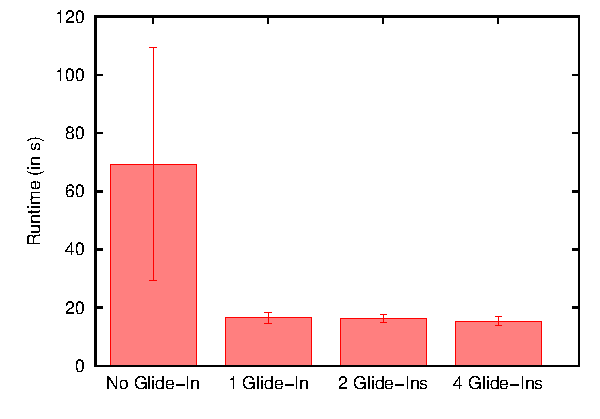
\includegraphics[width=0.5\textwidth]{perf_glidein.pdf}
        \caption{SAGA Glide-In Performance: The figure shows the average runtime of a 
        RE simulation with 16 RE processes running on 16 cores each on QueenBee. 
        The Glide-In framework provides the possibility to effectively cluster
        RE jobs to receive a significant reduced time to solution (upto 80\,\%) 
        even on a single machine.}

        % 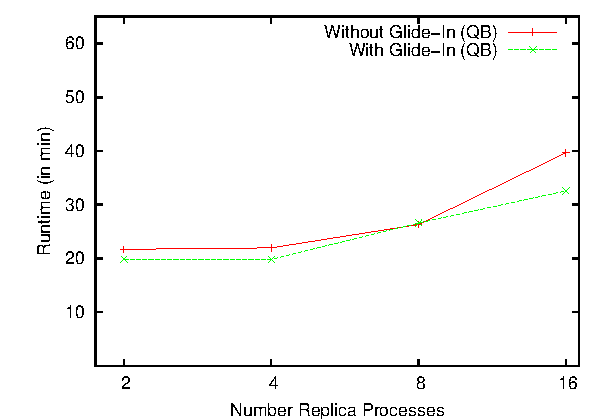
\includegraphics[width=0.5\textwidth]{perf_remd_glidin.pdf}
        % \caption{SAGA Glide-In Performance: The usage of the SAGA
        %   Glide-In provides a significant reduced time to solution
        %   even on a single machine in particular with more than 8
        %   replica jobs.}
    \label{fig:perf_remd_glidin}
\end{figure}

Figure~\ref{fig:perf_remd_glidin} shows that the SAGA Glide-In framework can provide
a reduced time to solution even on a single machine by avoiding queuing times for 
every sub-job and allowing the efficient dispatching of RE tasks solely through the 
Replica-Agent. During our experiments we were able to measure speedups of up to 80\,\%.

The unpredictable nature of these queueing times is reflected in the high standard deviation 
observed in the runtimes. While queueing times also have an impact on Glide-Ins, these are in general less
severe.  Further, for the Glide-In scenario, the queueing times become negligible, 
the longer the RE simulation is (the runtimes have been
kept short for this simple scenario). In contrast, when no Glide-Ins are used every sub-jobs 
is subject to the queuing delay at the local scheduler.

% old revision
% By avoiding long queuing time for big jobs, a distribution of the
% replica processes to a set of less crowded resources provides a lot of
% benefits.

In certain situation the usage of smaller jobs can have an advantage, 
e.\,g.\ when the local scheduler backfills such jobs. However, usually not all replica processes can be
backfilled -- the more processes are spawned the more likely are delays. 

The framework has also been deployed on multiple resources concurrently. This is in particular useful
for smaller resources, such as Oliver, where it is only possible to request 64 cores at a
time. In contrast to the QB only run, the runtime only slightly increases by about 1.5 minutes, which is 
acceptable compared to a possible delay due to insufficient resources on Poseidon.

The results can be summarized as follows: 1) The SAGA Glide-In framework can 
efficiently dispatches RE sub-jobs providing an enhanced time to solution even 
when deployed on a single machines. 2) By using a clever assignment of 
Glide-Ins to hosts and jobs, the runtime can 
be further optimized. In future, we plan to utilize this by deploying 
adaptive optimization strategies at runtime.

% The more processes are spawned, the more likely are
% such delays. While with the SAGA Glide-In framework the runtime only modestly increase 
% with more than 8 replicas, the runtime rapidly rises when using regular Globus job
% for spawning NAMD tasks. 
% By avoiding long queuing time for big jobs, a distribution of the replica processes to a set 
% of less crowded resources provides a lot of benefits.



\section{Any Other Applications}

 -- Data parallel applications

\section{Take Home Message}

\begin{itemize}

\item SAGA provides the abstractions and the ability to create
  multi-tasks applications that can exploit multiple and different
  infrastructure types.  We have demonstrated this via the
  implementation of two distinct, specific applications but both
  representative of a broader class of applications and running them
  in two different execution environments without changing the
  application in any way!The specific applications differed not only
  in the types of sub-tasks (homogenous versus heterogenous) but also
  in the nature of the coupling between the sub-tasks.
  

\item Not only do we need support for different programming models, 
this is also proof of support for agile execution models.


\item It is interesting to note that ``simple, naive'' implementations
  of these applications are possible; these would have these
  applications being developed as ``grid-unaware'' applications.
  Although we don't provide details here, the power of these
  applications arise from their ability to have an agile execution
  model, i.e., by being adaptive to dynamics resource requirements or
  availabiliy. In order to develop these applications such that they
  have agile execution models, these applications need to be
  grid-aware, ie explicitly control the distributed aspects. We
  believe explicit control is a critical for adaptive applications and
  posit that SAGA provides an important mechanism to implement the
  distributed features explicitly.

\end{itemize}







% \Section{Introduction}
%   There exist several applications which require several smaller but
%   heterogenous tasks to be solved in multiple-stages as part of the
%   overall solution.  Often the time-to-solution is the single most
%   important metric.  Distributed resources can thus help, especially
%   when combined with opportunistic scheduling/execution.  However, the
%   desire/need to use distributed computing comes with its own/unique
%   set of challenges.
  
%   We discuss three application types that are in turn composed of
%   multiple, smaller but {\it loosely-coupled} tasks -- Replica
%   Dynamics, Satisfiability problems, and Kalman filtering
%   applications.  Although these applications types are similar in that
%   they are comprised of multiple, smaller tasks, they are different in
%   that the individual sub-tasks are dissimilar for different reasons.
  
%   These application types are often multi-staged, with varying levels
%   of dependency between the stages. There could be, strict ordering
%   between the stages, ie. if all tasks in a stage must complete and be
%   globally synchronised before the next stage can begin. Thus there is
%   coupling between tasks within a given stage, and there is coupling
%   between stages.

%   Other challenges that any many-task system will encounter are: (i)
%   scheduling these sub-tasks is a challenge, (ii) level of speculative
%   computing that can be employed.

%   In parallel replica dynamics, the replicas can run for different
%   time durations between different stages. In replica-exchange
%   dynamics, the number and frequency of exchanges can vary.  Different
%   stages of this application vary; in other words, there is
%   time-domain heterogenity.

%   In Kalman filter based applications, the number and size of 
%   tasks between different stages varies. 

%   In the general class of satisfiability-based applications, as well
%   as the learning-based algorithms, there are elements of both kinds
%   of heterogenity between stages. GridSAT is an interesting example.
         
%\newpage
                  
\section*{Acknowledgement}
This work would not have been possible without the efforts and support
of the wider SAGA team. Important funding for SAGA specification and
development has been provided by the UK EPSRC grant number
GR/D0766171/1.  SJ acknowledges the e-Science Institute, Edinburgh for
supporting the research theme, ``Distributed Programming
Abstractions''.  This work has also been made possible thanks to the
internal resources of the Center for Computation \& Technology (CCT)
at Louisiana State University and computer resources provided by LONI.


\bibliographystyle{IEEEtran}
\bibliography{saga,literatur}
\end{document}


